\documentclass{article}

% ------------------------------ 76 characters -----------------------------
\usepackage[l2tabu, orthodox]{nag}

% -- Texto e codificação
\usepackage[utf8]{inputenc}
\usepackage[portuguese]{babel}
\usepackage{microtype}
\usepackage{xcolor}

% -- Tipo de letra
\usepackage{heuristica}
\usepackage[heuristica,vvarbb,bigdelims]{newtxmath}
\usepackage[T1]{fontenc}
%\renewcommand*\oldstylenums[1]{\textosf{#1}}

%\usepackage{lmodern}
%\usepackage[T1]{fontenc}

% -- Definir margens do documento
\usepackage{geometry}
\geometry{verbose, nomarginpar,
    tmargin = 2.5cm,
    bmargin = 2.5cm,
    lmargin = 2.5cm,
    rmargin = 2.5cm}
%\usepackage{showframe}

% -- Cabeçalho e rodapé
\usepackage{fancyhdr}
\fancyhf{}
\fancyhead[L]{\textsc{Header}}
\fancyhead[R]{\textsc{Footer}}
\fancyfoot[C]{\thepage}
\pagestyle{fancy}

% -- Funções matemáticas extra
\usepackage{mathtools}
\usepackage{siunitx}

% -- Símbolos extra
\usepackage{amssymb}
\usepackage{textcomp}
\usepackage{gensymb}
\usepackage{cancel}

% -- Referências
\usepackage{hyperref}

% --  Definições de imagens
\usepackage{graphicx}
\graphicspath{{graphics/}}
\usepackage{caption}
\usepackage{subcaption}

% -- Desenhar circuitos elétricos e lógicos
\usepackage{tikz}
\usepackage{pgfplots}
\usetikzlibrary{arrows.meta,positioning}
\pgfplotsset{compat=1.5}
\pgfplotsset{table/search path = {data}}
\pgfplotsset{	/pgf/number format/use comma,}

\begin{document}

\thispagestyle{empty}



\includegraphics[viewport=9.5cm 11cm 0cm 0cm,scale=0.29]{IST_A_CMYK_POS}
	
\begin{center}
	\vspace{70mm} % --  Espaço em branco
	\rule{\linewidth}{0.5pt} \\
    \vspace{2mm}
	\Huge \textsc{Projecto de Sistemas de Navegação} \\
	\rule{\linewidth}{2pt} \\
	\vspace{8mm} % -- Espaço em branco
	\LARGE Desenvolvimento de um sistema de detecção de intrusão em áreas restritas baseado em GPS diferencial
	
	\vspace{\fill} % --  Espaço em branco variável
	
	\normalsize
	\begin{tabular}{r l}
		Tiago \textsc{Matias} & \textbf{65655} \\
		João \textsc{Manito} & \textbf{73096} \\
		Daniel \textsc{de Schi}{\footnotesize FF}\textsc{art} & \textbf{81479}
	\end{tabular}
	
	\vspace{10mm} % --  Espaço em branco
	\Large Instituto Superior Técnico \\
	Mestrado em Engenharia Aeroespacial \\
	\vspace{1mm}
	\large Sistemas de Navegação
	
	\vspace{10mm} % --  Espaço em branco
	\Large Junho de 2018
\end{center}

\newpage

\section{Objectivo}

O objetivo do projeto é a implementação de um sistema de
posicionamento global derivado do GPS com correções baseadas em
estações locais, um sistema comummente apelidado de GPS diferencial,
ou DGPS, e a utilização desse mesmo sistema para detetar intrusão em
áreas pré-especificadas.

\section{Funcionamento}

Neste projeto implementámos melhoramentos de GPS através do método
conhecido como GPS diferencial. O GPS diferencial é um sistema para
corrigir a posição retornada por um recetor GPS convencional, utilizando um recetor de posição fixa pré-determinada para
calcular erros nos \textit{pseudoranges} em tempo real.

\subsection{GPS Diferencial}\label{diferential_theory}

A correção é realizada nos valores dos \textit{pseudoranges}
calculados pelo recetor local através dos satélites do sistema GPS.
Estes erros, que advêm do facto da influência da atmosfera no sinal
de GPS não ser constante, são calculados pela diferença dos
\textit{pseudoranges} da estação fixa e a distância real desta aos
satélites, cuja posição é conhecida pois esta está presente no sinal
de GPS. Uma vez calculados estes erros, estes são transmitidos ao
recetor local e subtraídos aos \textit{pseudoranges} calculados por
este. Calcula-se então a posição utilizando o método de GPS, mas
utilizando desta vez os \textit{pseudoranges} corrigidos.

Sendo $d_{GS}$ a distância entre o satélite $N$ e a
estação local, e $\rho_{GS}$ o \textit{pseudorange} obtido nesta, temos,
para cada satélite, o erro $e$ na equação \ref{sat_error}.
\begin{gather} \label{sat_error}
	\left[\begin{matrix}
		e^{(1)} \\
        e^{(2)} \\
        \vdots \\
        e^{(N)} \\
	\end{matrix}\right]
	= \left[\begin{matrix}
		d^{(1)}_{GS} - \rho^{(1)}_{GS} \\
        d^{(2)}_{GS} - \rho^{(2)}_{GS} \\
        \vdots \\
        d^{(N)}_{GS} - \rho^{(N)}_{GS} \\
	\end{matrix}\right]
\end{gather}
Sendo $\rho^{(N)}_{r}$ o \textit{pseudorange} obtido pelo receptor local, temos $\rho*_r $ como o valor corrigido para o receptor local do \textit{pseudorange}, na equação \ref{new_range}.
\begin{gather} \label{new_range}
	\left[\begin{matrix}
		\rho*^{(1)}_r \\
        \rho*^{(2)}_r \\
        \vdots \\
        \rho*^{(N)}_r \\
	\end{matrix}\right]
	= \left[\begin{matrix}
		\rho^{(1)}_{r} - e^{(1)} \\
        \rho^{(2)}_{r} - e^{(2)} \\
        \vdots \\
        \rho^{(N)}_{r} - e^{(N)} \\
	\end{matrix}\right]
\end{gather}
Com estes novos \textit{pseudoranges} podemos calcular a posição do receptor local da mesma forma que seria calculada no caso de GPS normal.

\subsection{Verificação de Intrusão de Área}

Para determinar a intrusão de um ponto em áreas restritas, foram
formuladas equações com base nas coordenadas ECEF calculadas pelo
DGPS. Estas equações foram formuladas para três tipos de volumes
geométricos distintos: esfera, cilindro e paralelepípedo (caixa).

\subsubsection{Esfera}

O cálculo da intrusão num volume esférico com base em coordenadas
ECEF foi de relativa facilidade, e foi consequentemente a primeira a
ser implementada. Fornecendo um ponto $(x_c,y_c,z_c)$ para o centro
da esfera e um raio $r$, para uma coordenada $(x_r,y_r,z_r)$
fornecida pelo recetor, podemos formular que o ponto está dentro da 
esfera se
\begin{gather*}
	\left\lVert(x_c,y_c,z_c) - (x_r,y_r,z_r)\right\rVert \leq r
\end{gather*}

\subsubsection{Cilindro}

A implementação do cilindro foi feita através de um ponto $(x_b,y_b,
z_b)$ correspondente à base, um raio da base $r$, e uma altura $h$.
A verificação da intrusão foi feita utilizando uma fatia circular do
cilindro com a mesma altura em LLH. Utilizando o centro desta mesma fatia
$(x_f,y_f,z_f)$, formula-se que o ponto está dentro do cilindro se
\begin{gather*}
	\left\lVert(x_f,y_f) - (x_r,y_r)\right\rVert \leq r\\
    z_f = z_r
\end{gather*}

\subsubsection{Paralelepípedo}

A última implementação foi a do paralelepípedo, que foi a menos trivial a
realizar. O algoritmo de deteção utilizado requer um paralelepípedo
recto. Para tal, trabalhou-se no sistema de coordenadas ENU, que é um sistema cartesiano.
Utilizando dois pontos $P_1$ e $P_3$ e a altura $h$ do
paralelepípedo obtiveram-se oito pontos que definem o paralelepípedo,
como se observa na figura \ref{fig:box}.

%if dot(u_ENU,xyz_ENU)>=dot(u_ENU,corners_ENU(1,:)) && dot(u_ENU,xyz_ENU)<=dot(u_ENU,corners_ENU(2,:))
%    if dot(v_ENU,xyz_ENU)>=dot(v_ENU,corners_ENU(1,:)) && dot(v_ENU,xyz_ENU)<=dot(v_ENU,corners_ENU(4,:))
%        if dot(w_ENU,xyz_ENU)>=dot(w_ENU,corners_ENU(1,:)) && dot(w_ENU,xyz_ENU)<=dot(w_ENU,corners_ENU(5,:))

\begin{figure}[ht]
	\centering
	\begin{tikzpicture}[ppoint/.style = {circle,draw,inner sep = 0pt, minimum size = 3pt}]
		\node (p1) at (0,0) [ppoint,label = {135:$P_1$}] {};
        \node (p2) at (1,1) [ppoint,label = {135:$P_2$}] {};
        \node (p3) at (3,1) [ppoint,label = {135:$P_3$}] {};
        \node (p4) at (2,0) [ppoint,label = {135:$P_4$}] {};
        \node (p5) at (0,3) [ppoint,label = {135:$P_5$}] {};
        \node (p6) at (1,4) [ppoint,label = {135:$P_6$}] {};
        \node (p7) at (3,4) [ppoint,label = {135:$P_7$}] {};
        \node (p8) at (2,3) [ppoint,label = {135:$P_8$}] {};
        \draw (p1) -- (p5) -- (p6) -- (p7) -- (p3) -- (p4) -- (p1);
        \draw (p5) -- (p8) -- (p7) (p8) -- (p4);
        \draw [dashed] (p1) -- (p2) -- (p6) (p2) -- (p3);
        \draw [<->] (p3) ++(0.5,0) -- node [auto,swap] {$h$} ++(0,3);
	\end{tikzpicture}
    \caption{Relação entre os pontos do paralelepípedo.}
    \label{fig:box}
\end{figure}

Utilizando um ponto do recetor $P_r = (x_r,y_r,z_r)$, as condições de
intrusão podem ser definidas extraindo três vetores $u$, $v$ e $y$ do
paralelepípedo.
\begin{gather*}
	u = P_1 - P_2 \\
    v = P_1 - P_4 \\
    w = P_1 - P_5
\end{gather*}

Com isto definido, o ponto do recetor pode ser considerado dentro do
paralelepípedo quando todas as condições das equações \ref{eq:box_condu},
\ref{eq:box_condv} e \ref{eq:box_condw} são correspondidas.
\begin{gather}
	\label{eq:box_condu}
	u \cdot P_1 \leq u \cdot P_r \leq u \cdot P_2 \\
    \label{eq:box_condv}
    v \cdot P_1 \leq v \cdot P_r \leq v \cdot P_4 \\
    \label{eq:box_condw}
    w \cdot P_1 \leq w \cdot P_r \leq w \cdot P_5
\end{gather}

\subsection{Determinação da posição do receptor}

De forma a poder implementar este algoritmo, foi necessário utilizar um receptor de GPS que permita obter os \textit{pseudoranges}, uma vez que o formato NMEA não disponibiliza esses dados. Para o efeito foram usados dois receptores \textit{ublox} EVK-6T. 

Usando a informação das especificações \texttt{IS-GPS-200H} e texttt{u-blox 6 Receiver Description}, foi criado um algoritmo que processa as mensagens do receptor (nomeadamente as mensagens RXM-RAW, AID-EPH e AID-HUI). Em seguida foram usados os \textit{pseudoranges}, os dados dos satélites e os parâmetros de correção para obter uma estimativa da posição do receptor usando o método de \textit{least squares}.

\section{Implementação e Resultados}

A implementação do DGPS foi realizada com recurso ao MATLAB,
reutilizando parte do código desenvolvido ao longo do semestre nas
aulas da unidade curricular. Numa instância inicial, foram
utilizados dados fornecidos pelo professor para as posições dos
satélites e para os \textit{pseudoranges} de alguns satélites,
obtidos através da estação GNSS colocada no topo do Instituto de
Telecomunicações, como descrita no documento
\texttt{AntennaSurvey.pdf}. Usando esses dados, foi criado um algoritmo de processamento dos mesmos, de forma a converter a informação fornecida pelo receptor de GPS em formatos mais fáceis de utilizar. Posteriormente, esse algoritmo foi usado para determinar os \textit{pseudoranges} dos receptores, que depois foram usados para obter as correções de DGPS. Para a detecção de intrusão, não foi possível utilizar dados de \textit{pseudoranges} reais devido a restrições de tempo. No entanto, validou-se o seu funcionamento utilizando um receptor de GPS com saída NMEA de um \textit{smartphone}.

\subsection{Processamento de mensagens de GPS e determinação da posição das estações base}

Numa primeira fase, fez-se apenas pós-processamento de dados obtidos pelo receptor em uso.  Este receptor apresenta um conjunto de mensagens possíveis na sua especificação, pelo que se optou apenas por processar três tipos de mensagens: 
\begin{itemize}
  \item RXM-RAW, que disponibiliza informação de \textit{pseudoranges} dos vários satélites em uso, bem como um \textit{timestamp} da medição;
  \item AID-EPH, que disponibiliza informação de efemérides para os vários satélites, bem como informações de integridade dos mesmos;
  \item AID-HUI, que disponibiliza informação relativa a parâmetros de correção para os relógios e ionosfera.
\end{itemize}

Recorrendo aos documentos  \texttt{IS-GPS-200H} e \texttt{u-blox 6 Receiver Description}, foi criada uma rotina de processamento de dados, que converte o conteúdo de cada mensagem num formato predefinido, igual ao usado no decurso da UC.

De seguida, foram determinadas as posições dos satélites e calculada a posição do receptor usando o método de \textit{Least Squares}. Corrigindo o efeito do  \textit{clock bias} e sincronismo dos relógios de GPS, bem como das perturbações troposférica e ionosférica, foi obtida uma estimativa mais precisa para a posição do receptor. Tendo ignorado todas as posições em que o parâmetro PDOP é superior a 4, foi obtida uma estimativa para a posição do receptor. Este processo foi realizado para os dados fornecidos na página da UC (ficheiros \texttt{ub1.ubx.1744.327600} e \texttt{ub2.ubx.1744.327600}), bem como para um conjunto de dados obtido com o receptor supramencionado.

As posições determinadas são então:
\begin{table}[h]
\centering
\begin{tabular}{ c | c | c | c }
 Receptor & Latitude (º) & Longitude (º) & Altitude (m)  \\
 \hline
 UB1 & 38.7375691156866 & 9.13852429667141 & 219.265118060666  \\
 UB2 & 38.7376975066945 & -9.13853426280023 & 209.618087988563  \\
\end{tabular}
\caption{Posição determinada dos receptores em coordenadas LLH.}
\label{tabela1}
\end{table}

\begin{table}[ht]
\centering
\begin{tabular}{ c | c | c | c }
 Receptor & X (m) & Y (m) & Z (m)  \\
 \hline
 UB1 & 4918548.05800941 & -791216.081612259 & 3969771.54527795  \\
 UB2 & 4918531.68520011 & -791214.325497741 & 3969776.62639603  \\
\end{tabular}
\caption{Posição determinada dos receptores em coordenadas ECEF.}
\label{tabela2}
\end{table}

\begin{table}[ht]
\centering
\begin{tabular}{ c | c  }
 Receptor & Erro médio (m)  \\
 \hline
 UB1 & 26.4846310745313  \\
 UB2 & 30.2741811841672  \\
\end{tabular}
\caption{Erro médio da posição dos receptores.}
\label{tabela3}
\end{table}

\begin{figure}[!ht]
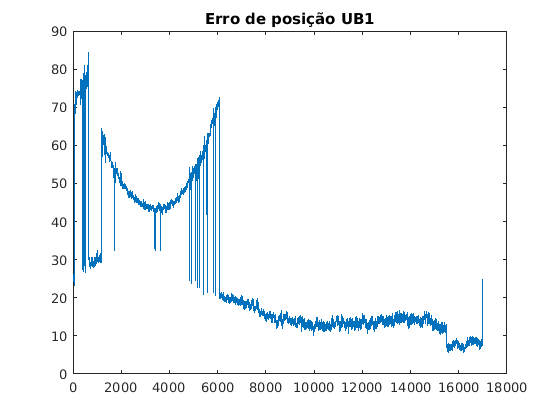
\includegraphics[width=0.49\textwidth]{erro_posicao_UB1}
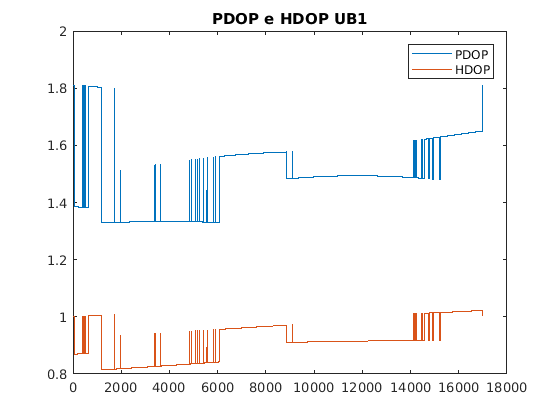
\includegraphics[width=0.49\textwidth]{UB1_PDOP_HDOP}
\caption{Evolução do erro de posição absoluto, PDOP e HDOP do receptor instalado em UB1 ao longo do período de amostragem.}
\label{fig:erro_simples_UB1}
\end{figure}

\begin{figure}[!ht]
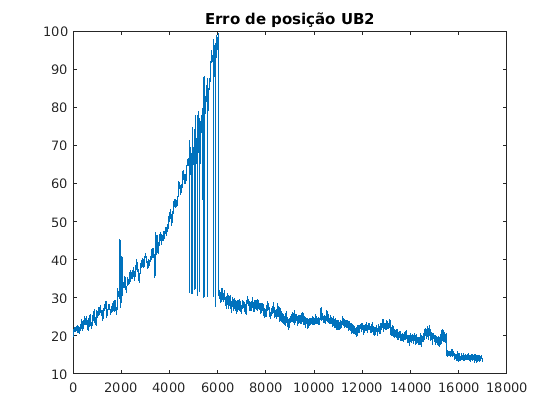
\includegraphics[width=0.49\textwidth]{erro_posicao_UB2}
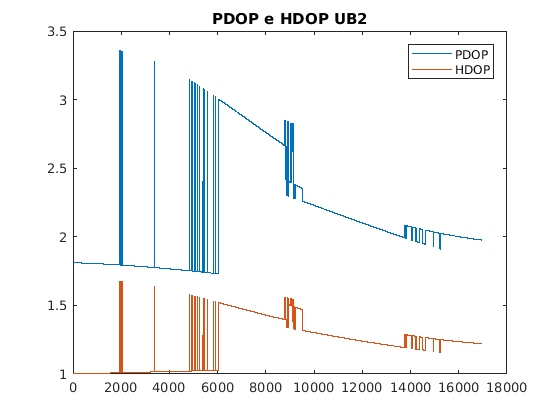
\includegraphics[width=0.49\textwidth]{UB2_PDOP_HDOP}
\caption{Evolução do erro de posição absoluto, PDOP e HDOP do receptor instalado em UB2 ao longo do período de amostragem.}
\label{fig:erro_simples_UB2}
\end{figure}

\newpage
Dos gráficos, podemos verificar que existe uma zona de elevado erro na posição, comum a ambos os receptores. Embora a causa concreta não tenha sido identificada, presumimos que seja devido a algum erro na nossa implementação. O valor médio foi algo afetado por este fenómeno, tal como se pode verificar no erro médio. Para os gráficos de PDOP e HDOP, verificamos que estes apresentam valores não muito elevados, no caso de UB2, e dentro da gama [0;2.5] no caso de UB1. Há no entanto uma certa correlação entre certos pontos dos gráficos de DOP e erro, em que em tempos semelhantes existem desvios dos valores esperados. Tal dever-se-á possivelmente ao erro de implementação acima referido.

Os resultados desta parte do projecto podem ser obtidos usando o \textit{script} \texttt{determinacao\_receptores.m}.






\newpage

\subsection{Determinação das correções diferenciais para os receptores}
Como teste do funcionamento do modo diferencial, foram usados os dados dos dois receptores, um como estação base e o outro como receptor móvel. 
Usando o algoritmo da secção \ref{diferential_theory}, e recorrendo a algumas alterações ao mesmo de forma a contabilizar as diferenças de \textit{clock bias} entre receptores e outras correções, obtivemos uma estimativa para a posição do receptor UB2, tendo como estação base o receptor UB1.

\begin{figure}[ht]
\centering
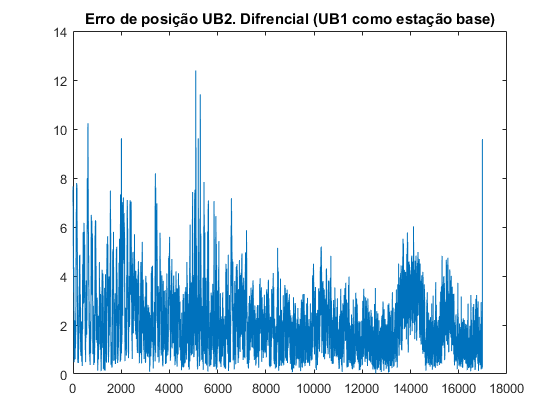
\includegraphics[width=0.5\textwidth]{dif_RF2}
\caption{Evolução do erro de posição absoluto de UB2 em modo diferencial ao longo do período de amostragem, tendo como estação base.}
\label{fig:erro_simples_UB2_diff}
\end{figure}

Desta figura verificamos que existe um erro claramente inferior ao do método anterior, pelo que podemos afirmar que o método de correção diferencial funciona. É especialmente notável que o comportamento errático presente nas primeiras 6000 amostras analisadas com o método anterior foi completamente anulado, o que reforça a ideia de que a correção diferencial é muito mais robusta que a determinação de posição usando apenas um receptor. No entanto o erro ainda é algo elevado, pelo que há claramente trabalho a desenvolver para permitir reduzir este erro.

Relativamente aos parâmetros PDOP e HDOP, devido a problemas com o código não foi possível calcular os seus valores.

Os resultados desta parte do projecto podem ser obtidos usando o \textit{script} \texttt{determinacao\_diferencial.m}.





\subsection{Detecção de intrusão}
A última parte deste projecto consiste na aplicação dos algoritmos e código desenvolvidos nas secções anteriores e aplicá-los a um algoritmo que determine se o receptor se encontra dentro da área restrita ou não. Infelizmente, por restrições de tempo não nos foi possível utilizar a determinação de posição usando DGPS para este efeito. Assim, recorremos ao uso de dados NMEA para essa detecção, de forma a validar o algoritmo de detecção. 

\begin{figure}[!ht]
\centering
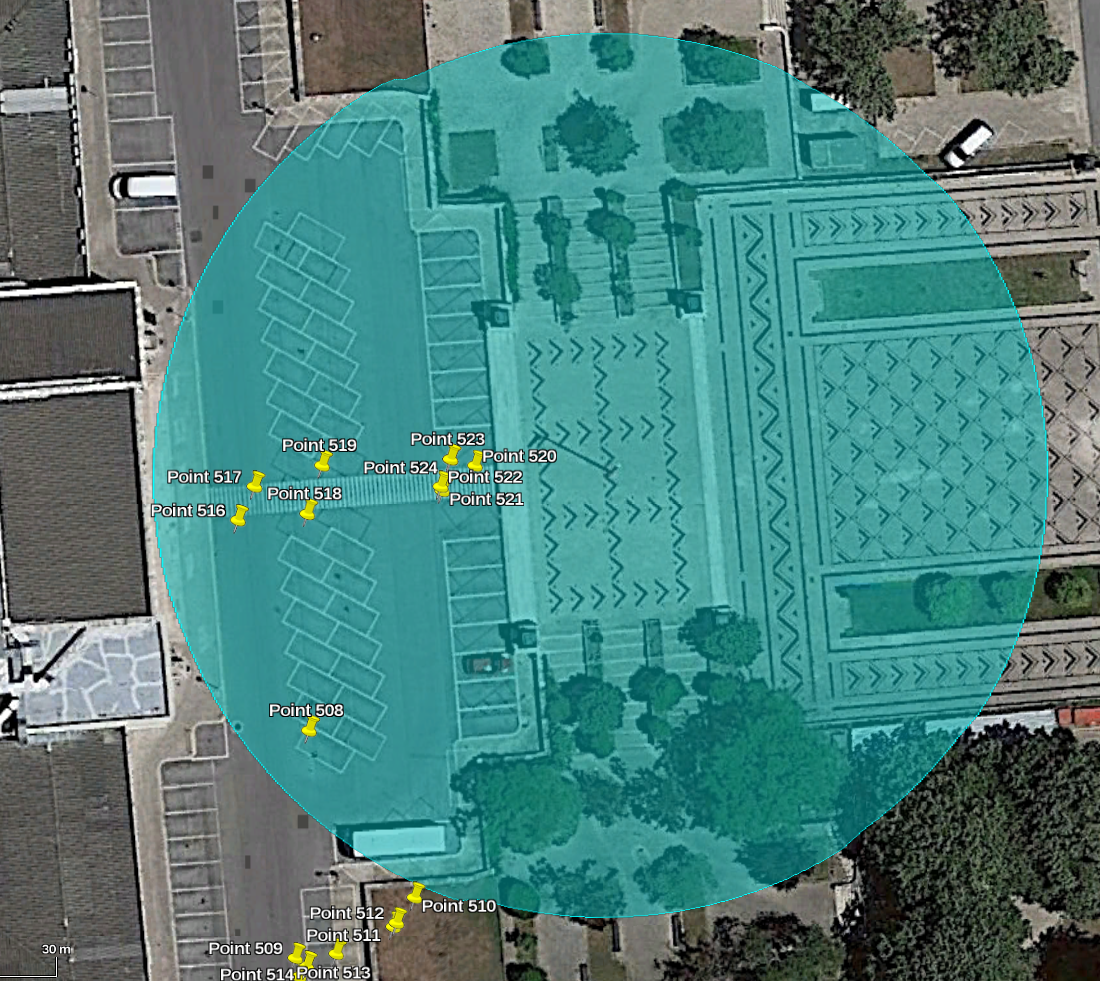
\includegraphics[width=\textwidth]{spherical_projection}
\caption{Zona de intrusão esférica.}
\label{fig:erro_simples_UB1_sph}
\end{figure}

\newpage
Na região esférica (aqui representada como uma projecção em 2D) verificamos que o algoritmo detecta corretamente que o receptor de GPS se encontra dentro da zona restrita. Note-se também a falta do ponto 519, que, embora aparente estar dentro da região nesta projecção 2D, se encontra a uma altitude suficientemente elevada para estar fora da zona restrita. Os pontos que se encontram na zona restrita são então \{517, 518, 520, 521, 522, 523, 524\}.

\newpage

\begin{figure}[!ht]
\centering
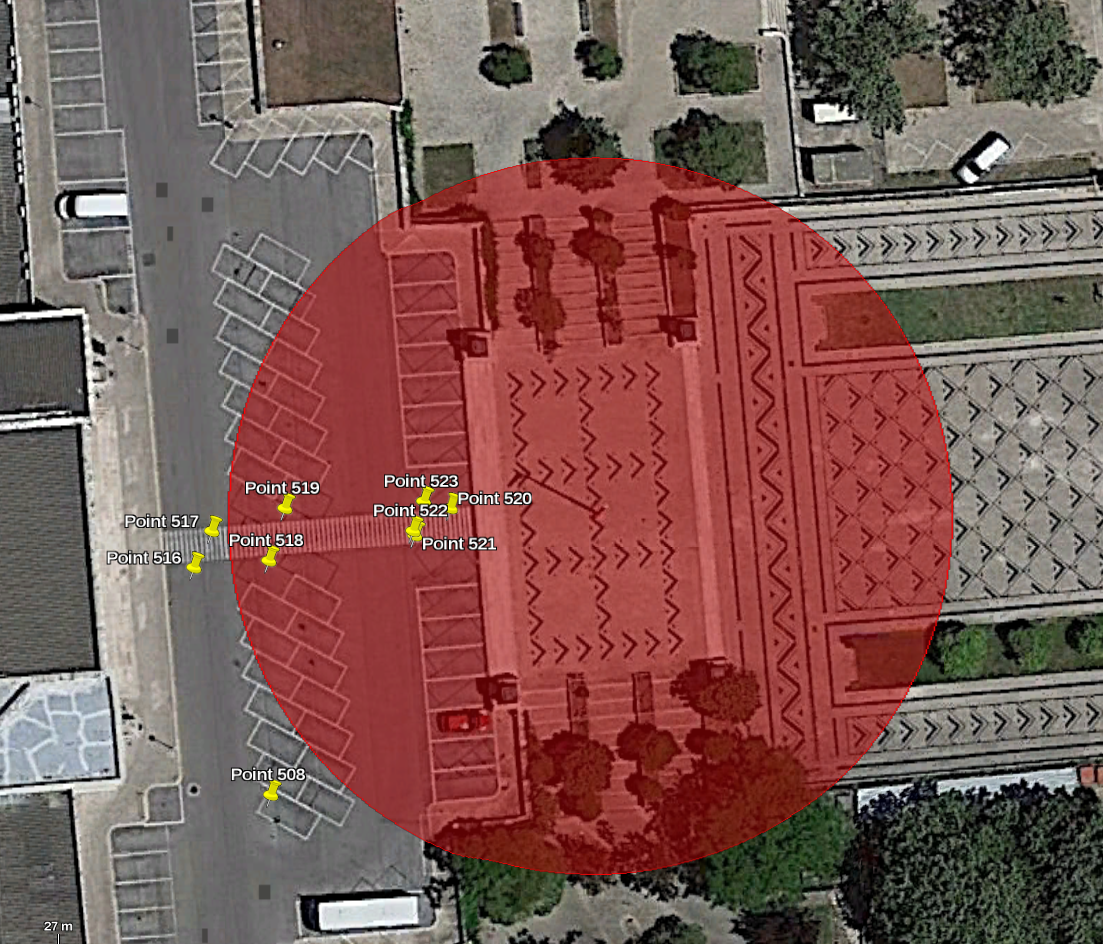
\includegraphics[width=\textwidth]{cylindrical_projection}
\caption{Zona de intrusão cilíndrica.}
\label{fig:erro_simples_UB1_cyl}
\end{figure}
Na região cilíndrica (aqui representada como uma projecção em 2D) verificamos que o algoritmo detecta corretamente que o receptor de GPS se encontra dentro da zona restrita. Neste caso, devido à forma do cilindro, o ponto 519 já faz parte do conjunto de pontos na zona restrita, sendo estes \{518, 519, 520, 521, 522, 523, 524\}.

\newpage


\begin{figure}[!ht]
\centering
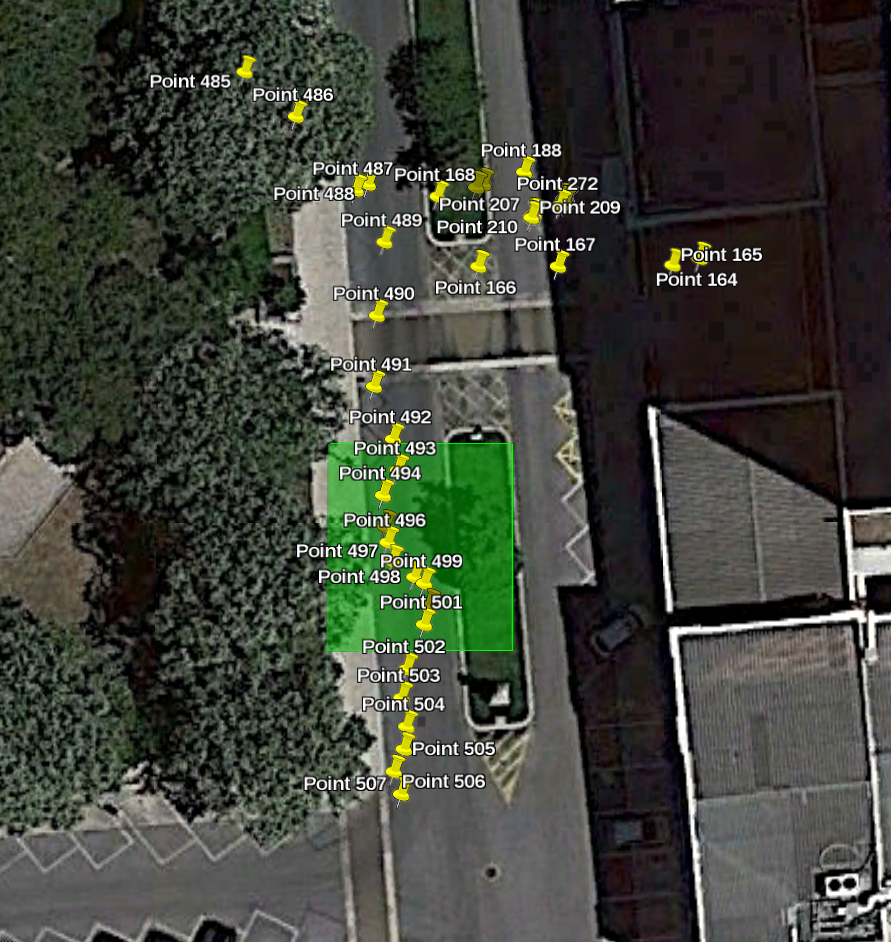
\includegraphics[width=\textwidth]{box_projection}
\caption{Zona de intrusão em paralelepípedo.}
\label{fig:erro_simples_UB1_box}
\end{figure}

Na região paralelepipédica, verificamos também que todos os pontos dentro da mesma são corretamente identificados, sendo o conjunto de pontos \{492, 493, 494, 495, 496, 497, 498, 499, 500, 501\}. 

Os resultados desta parte do projecto podem ser obtidos usando o \textit{script} \texttt{intrusion\_test.m}.

\newpage

\section{Conclusões}

Embora o projecto não tenha sido concluído (ficando a faltar a utilização do algoritmo de DGPS aplicado a receptores que não os instalados na torre bem como o funcionamento dos algoritmos em tempo real), foi-nos possível verificar que o algoritmo desenvolvido para DGPS apresenta uma redução do erro significativa relativamente à determinação de posição utilizando apenas um receptor de GPS. O erro obtido, embora ainda seja na ordem dos metros, já é pequeno o suficiente para considerar que este algoritmo, mesmo aplicado a um receptor de GPS com taxa de actualização de 1s, é viável para o objectivo principal do projecto, a detecção de intrusão, visto esta ser uma área em que o conhecimento da posição com precisão abaixo da ordem do metro é desnecessário.

Já relativamente ao algoritmo de detecção de intrusão, verificamos que, nos casos testados, este funciona de forma satisfatória, detectando correctamente os pontos em que há intrusão.

Embora não nos tenha sido possível a conclusão do projecto, consideramos que os resultados obtidos são satisfatórios, uma vez que mostram a viabilidade dos algoritmos desenvolvidos para o uso em questão.


\end{document}